\documentclass[a4paper, 11pt, oneside]{memoir}
\semiisopage

\chapterstyle{veelo}


%% ALTERNATIBAK / ALTERNATIVAS
%\chapterstyle{default}
%\chapterstyle{bianchi}
%\chapterstyle{brotherton}
%\chapterstyle{demo2}
%\chapterstyle{ell}
%\chapterstyle{ger}
%\chapterstyle{wilsondob}

\pdfobjcompresslevel 0


%% INFORMAZIOA / INFORMACIÓN %%
\newcommand{\egilea}{Iñaki Moreno Estebanez}
\newcommand{\zuzendariak}{
	Iñigo Perona Balda
}
\newcommand{\izenburua}{Detección de tráfico maligno mediante técnicas de
aprendizaje automático en sistemas IDS de red}
\newcommand{\data}{\today}


%% BAKARRIK BAT DESKOMENTATU, GRADU AMAIERAKO LANA BADA. BESTELA, DENAK KOMENTATU%%
%% DESCOMENTAR SOLO UNO SI ES UN TRABAJO FIN DE GRADO. SINO, COMENTAR TODOS%%

%\newcommand{\ikasketak}{Informatika Ingeniaritzako Gradua}
%\newcommand{\ikasketak}{Grado en Ingeniería Informática}
%\newcommand{\ikasketak}{Degree in Informatics Engineering}
%\newcommand{\ikasketak}{Adimen Artifizialeko Gradua}
\newcommand{\ikasketak}{Grado en Inteligencia Artificial}
%\newcommand{\ikasketak}{Degree in Artificial Intelligence}


%% BAKARRIK BAT DESKOMENTATU, INGENIARITZA INFORMATIKAKOA BADA. BESTELA, DENAK KOMENTATU %%
%% DESCOMENTAR SOLO UNO SI ES EN INGENIERÍA INFORMÁTICA. SINO, COMENTAR TODOS %%

%\newcommand{\espezialitatea}{Konputazioa}
%\newcommand{\espezialitatea}{Computación}
%\newcommand{\espezialitatea}{Computing}
\newcommand{\espezialitatea}{Software Ingeniaritza}
%\newcommand{\espezialitatea}{Ingeniería de Software}
%\newcommand{\espezialitatea}{Software Engineering}
%\newcommand{\espezialitatea}{Konputagailuen Ingeniaritza}
%\newcommand{\espezialitatea}{Ingeniería de Computadores}
%\newcommand{\espezialitatea}{Computer Engineering}

%% BAKARRIK BAT DESKOMENTATU MASTER AMAIERAKO LANA BADA. BESTELA, DENAK KOMENTATU%%
%% DESCOMENTAR SOLO UNO SI ES UN TRABAJO FIN DE MASTER. SINO, COMENTAR TODOS%%

%\newcommand{\ikasketak}{Máster Universitario en Ingeniería Computacional y Sistemas Inteligentes}
%\newcommand{\ikasketak}{Konputazio Ingeniaritza eta Sistema Adimentsuak Unibertsitate Masterra}

%% TESIENTZAKO KONFIGURATU
%\newcommand{\saila}{Department of Computer Science and Artificial Intelligence}
%\newcommand{\phdarloa}{Computer Science}
%% KOMENTATU A4 FORMATUAN ATERATZEKO, FORMATU TXIKIAGOAN AGERTZEKO 
%% GERO INPRIMATZEKO. MOZTEKO MARKAK IKUSTEKO GEHITU showtrims AUKERA
%% memoir KLASEAREN ARGUMENTUETAN
%\newcommand{\croppedsize}

%% DOKUMENTUAREN HIZKUNTZA / BAKARRIK BAT DESKOMENTATU %%
%% IDIOMA DEL DOCUMENTO / DESCOMENTAR SOLO UNO %%
%\newcommand{\euskaraz}{}
\newcommand{\castellano}{}
%\newcommand{\english}{}

\ifdefined\euskaraz
  \usepackage[eu]{ifcommands}
\else\ifdefined\english
  \usepackage[en]{ifcommands}
\else
  \usepackage[es]{ifcommands}
\fi\fi

\input config/macros

% Las figuras del TFG las genera scripts/figuras/ y viven fuera del
% directorio de la memoria, en PDF vectorial. Se anaden a graphicspath
% para poder citarlas por su nombre corto (F16_..., F19_...).
\graphicspath{{figures/}{../figuras/memoria/}}

% Pseudocodigo. `algorithm` da el flotante y `algpseudocode` el cuerpo. El
% rotulo de la lista viene en ingles por defecto, asi que se traduce.
% memoir ya define listofalgorithms; se libera para que el paquete pueda
% redefinirlo sin chocar.
\let\listofalgorithms\relax
\usepackage{algorithm}
\usepackage{algpseudocode}
\renewcommand{\listalgorithmname}{Índice de algoritmos}
\floatname{algorithm}{Algoritmo}
\renewcommand{\algorithmicrequire}{\textbf{Entrada:}}
\renewcommand{\algorithmicensure}{\textbf{Salida:}}
% Las palabras clave del pseudocodigo vienen en ingles por defecto.
\algrenewcommand{\algorithmicfor}{\textbf{para}}
\algrenewcommand{\algorithmicforall}{\textbf{para todo}}
\algrenewcommand{\algorithmicdo}{\textbf{hacer}}
\algrenewcommand{\algorithmicend}{\textbf{fin}}
\algrenewcommand{\algorithmicif}{\textbf{si}}
\algrenewcommand{\algorithmicthen}{\textbf{entonces}}
\algrenewcommand{\algorithmicelse}{\textbf{si no}}
\algrenewcommand{\algorithmicreturn}{\textbf{devolver}}
\algrenewcommand{\algorithmicwhile}{\textbf{mientras}}

% Al retirar los agradecimientos los numeros romanos del indice pasaron
% a cuatro cifras (viii) y la caja que memoir les reserva se queda 1,2 pt
% corta. Se ensancha; no afecta al resto del documento.
\setpnumwidth{2.2em}
\setrmarg{3.2em}



\title{\izenburua}
\author{\egilea}
\date{\data}


\begin{document}
 
%% AZALA BEREZIRIK BADUZU (PDF FORMATUAN), DESKOMENTATU%%
%% SI HAY UNA PORTADA ESPECIAL (EN PDF), DESCOMENTAR%%
	
%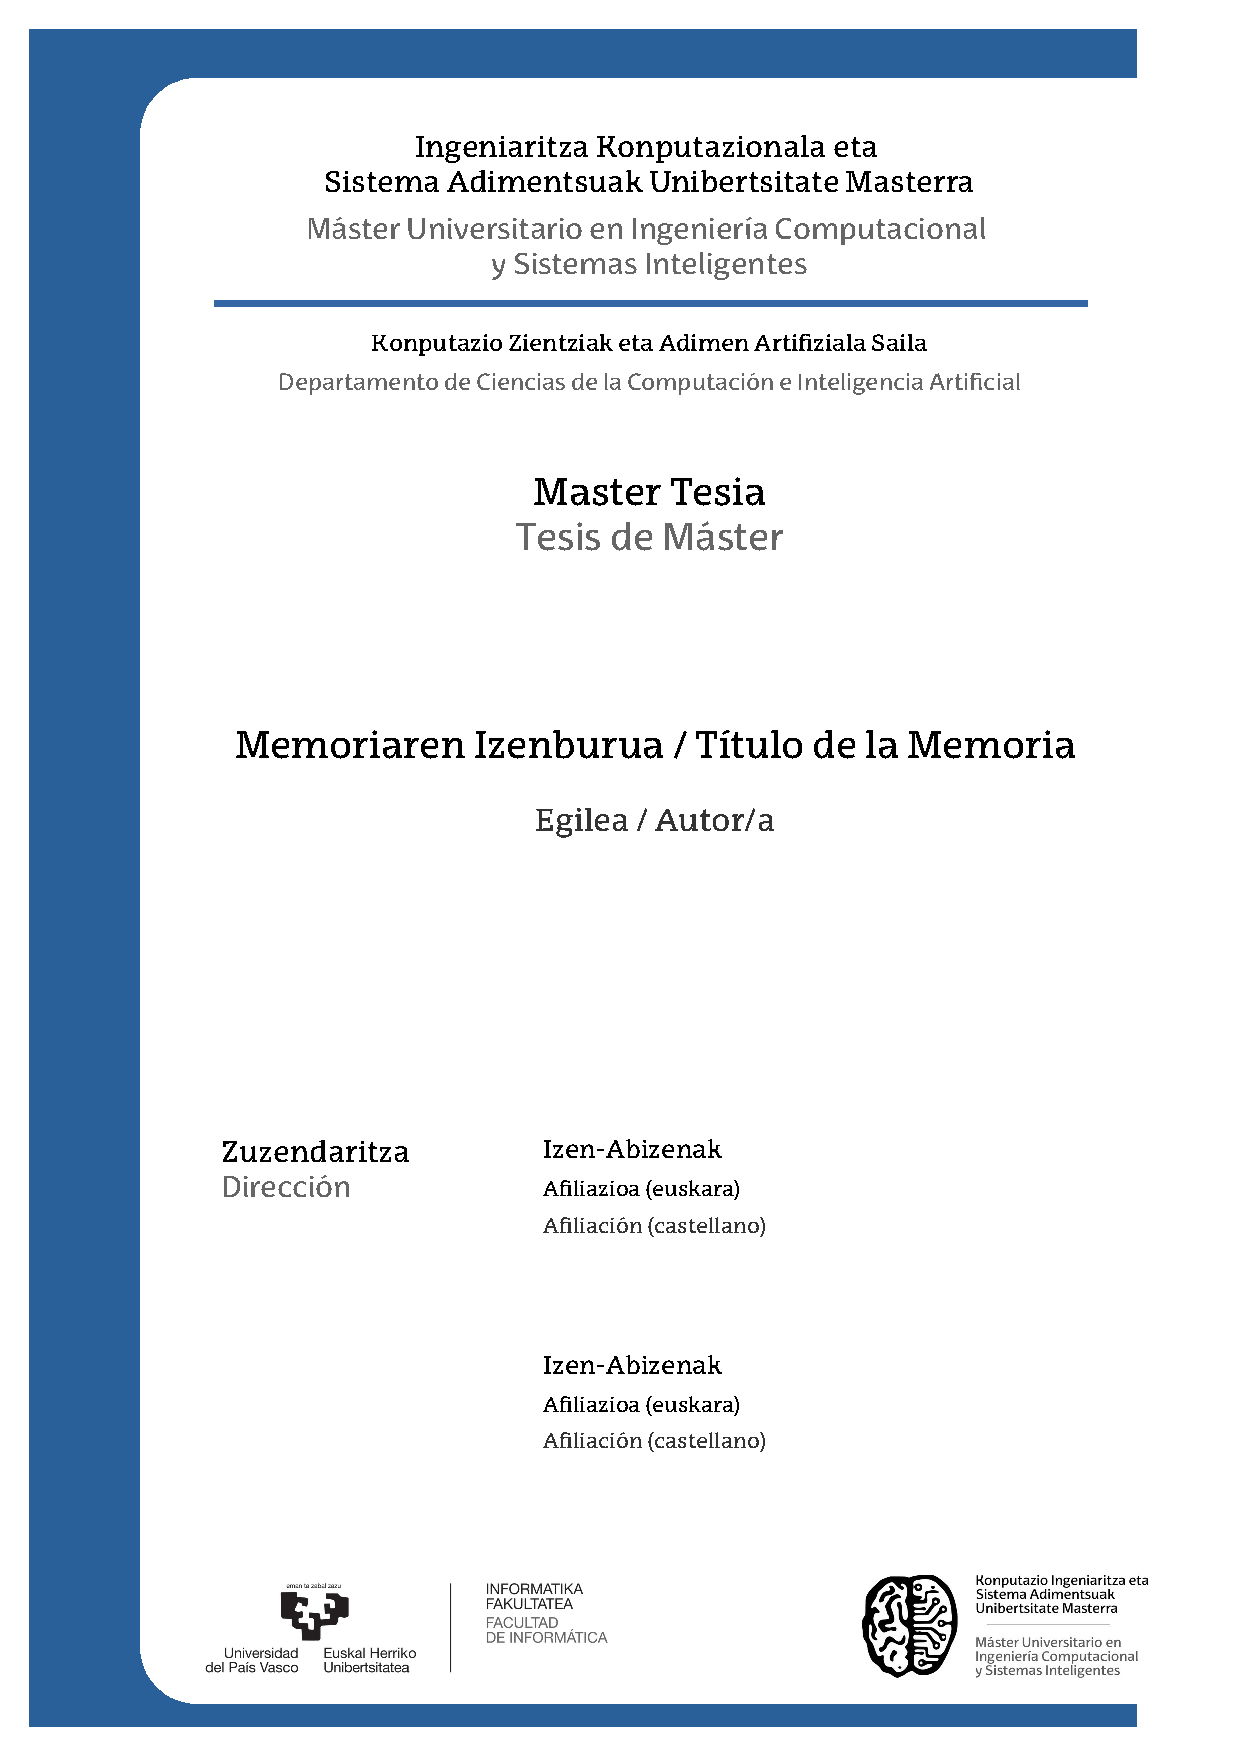
\includepdf[pages={1-}]{cover.pdf}
%\cleardoublepage
 
 
%% AUKERATU DAGOKIONA. AZALA BEREZIA GEHITUZ GERO, KOMENTATU DAITEKE, BETIERE HEMENGOAN AGERTZEN DEN INFORMAZIOA AGERTZEN BADA %%
%% SELECCIONA LA QUE CORRESPONDA. EN CASO DE TENER UNA PORTADA ESPECIAL SE PUEDE COMENTAR, SIEMPRE Y CUANDO DICHA PORTADA INCLUYA LA INFORMACIÓN QUE APARECE EN ESTA%%
 
%\input config/cover_informatika
\input config/cover_adimen_artifiziala
%\input config/cover_masterra
%\input config/cover_phd_dissertation
 
\cleardoublepage
\frontmatter
\aliaspagestyle{chapter}{plain}
\aliaspagestyle{cleared}{plain}
\pagestyle{plain}
\setcounter{page}{1}
 
%%%%%%%%%%%%%%%%%%%%%%%%%%%%%%%%
% ESKER ONAK / AGRADECIMIENTOS %
%%%%%%%%%%%%%%%%%%%%%%%%%%%%%%%%
 
%% KOMENTATU HIRU LERRO HAUEK ATALA NAHI EZ BADUZU
%% COMENTA ESTAS TRES LÍNEAS SI NO QUIERES ESTE APARTADO
% [Retirado: el autor no incluye agradecimientos.] \chapter*{Esker onak / Agradecimientos}
% Sin agradecimientos por decisión del autor. El fichero de la plantilla,
% que solo traía texto de ejemplo, se ha eliminado.
% \cleardoublepage
 
%%%%%%%%%%%%%%%%%%%%%%%
% LABURPENA / RESUMEN %
%%%%%%%%%%%%%%%%%%%%%%%
 
\chapter*{Resumen}
\input chapters/abstract
\cleardoublepage
 
\ifdefined\euskaraz
\chapter*{Garapen Jasangarrirako Helburuak} \label{ch:GJH}
\input chapters/GJH_ODS_SDG/GJH
\else\ifdefined\english
\chapter*{Sustainable Development Goals} \label{ch:SDG}
\input chapters/GJH_ODS_SDG/SDG
\else
\chapter*{Objetivos de Desarrollo Sostenible} \label{ch:ODS}
\input chapters/GJH_ODS_SDG/ODS
\fi\fi
 
\cleardoublepage
 
%%%%%%%%%%%%%%%%%%%%%%%%%%%%%%
% EDUKIEN ZERRENDA / ÍNIDCES %
%%%%%%%%%%%%%%%%%%%%%%%%%%%%%%
 
\openany
\pdfbookmark[1]{\contentsname}{toc}
\begin{KeepFromToc}
  \tableofcontents
\end{KeepFromToc}
\clearpage
\listoffigures
\clearpage
\listoftables
\clearpage
\listofalgorithms
\openany
 
%%%%%%%%%%%%%%%%%%%%%%
% EDUKIA / CONTENIDO %
%%%%%%%%%%%%%%%%%%%%%%
 
\cleardoublepage
\mainmatter
\pagestyle{ruled}
 
\chapter{Introducción} \label{ch:introduccion}
\input chapters/01_introduccion
\cleardoublepage

\chapter{Estado del arte} \label{ch:estado-del-arte}
\input chapters/02_estado_del_arte
\cleardoublepage

\chapter{Del PCAP al dataset: metodología} \label{ch:metodologia}
\input chapters/03_metodologia
\cleardoublepage

\chapter[La evaluación intra-día]{La evaluación intra-día: por qué no discrimina} \label{ch:regimenes}
\input chapters/04_regimenes
\cleardoublepage

\chapter{Generalización, calibración y robustez} \label{ch:generalizacion}
\input chapters/05_generalizacion
\cleardoublepage

\chapter{Conclusiones} \label{ch:conclusiones}
\input chapters/06_conclusiones
\cleardoublepage
 
%%%%%%%%%%%%%%%%%%%%%%%%%%%%
%% ERANSKINAK / APENDICES %%
%%%%%%%%%%%%%%%%%%%%%%%%%%%%
 
\addappheadtotoc
\appendix
 
\ifdefined\euskaraz
\chapter{AA sortzailearen erabilera deklarazioa} \label{ch:deklarazioa}
\input chapters/appendix/deklarazioa
\else\ifdefined\english
\chapter{Declaration of use of generative AI} \label{ch:declaration}
\input chapters/appendix/declaration
\else
\chapter{Declaración del uso de IA Generativa} \label{ch:declaracion}
\input chapters/appendix/declaracion
\fi\fi

\chapter{Resultados secundarios} \label{ch:anexo-resultados}
\input chapters/appendix/resultados_secundarios
 
 
%%%%%%%%%%%%%%%%%%
%% BIBLIOGRAFIA %%
%%%%%%%%%%%%%%%%%%
\bibliographystyle{unsrt}
\bibliography{erreferentziak}

 
\end{document}
